\section{Introduction}
\label{sec:introduction}
\subsection{Background}
\paragraph{}Research on Fuel cells started in 1801 when British Chemist Humphry Davy was setting up experiments to assist him in separating several materials using voltaic piles. The experiments set the background for the development of fuel cells which Christian Friedrich Schönbein worked on in 1838. Sir William Grove was the first scientist to prove that reaction between hydrogen and oxygen produced electricity in 1939. He carried out experiments on water electrolysers and fuel cells using his background on electrolysis to come up with a reverse process to generate electricity. He succeeded in building a device that combined water and hydrogen to generate electricity. The new device was originally called a gas battery, but later was renamed the fuel cell.
\paragraph{}The first operational fuel cell was developed by Charles Langer and Ludwig Mond. The duo developed a functional fuel cell, obtaining fuel capacity of 0.73V at 20A/m2. Francis Bacon advanced the Mond and Langer fuel cell in 1958, which was later used in the Apollo mission in 1969. Since then, the space agencies have been using fuel cells to power the space crafts and provide water for the astronauts.
\begin{figure}
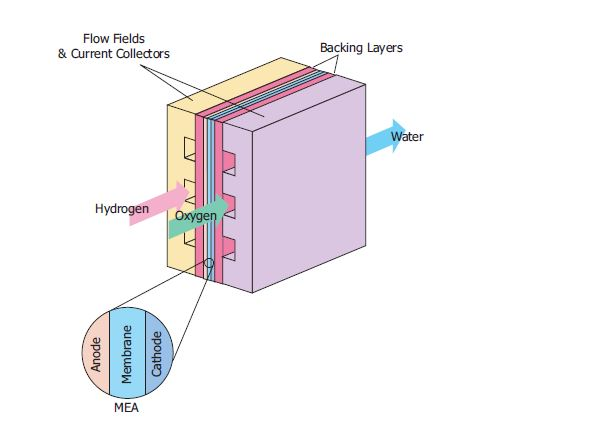
\includegraphics{Figures/Figure3}
\caption{Fuel Cell Structure
\cite{pukrushpan_modeling_2003}}
\end{figure}

\paragraph{}With the current global challenge in the energy sector, there is an increasing need for power generation with minimal pollution and environmental degradation. As a way of mitigating environmental pollution and providing energy shortage routes, Fuel Cell technologies have been considered as elements of alternative energy systems. These technologies capitalize on high efficiencies (between 50–65 percent, Supramaniam, et al., 1999 \cite{ashby_fuel_nodate}) and low emissions.
\paragraph{}Fuel cells are increasingly becoming a promising alternative to internal combustion engines (ICEs) and thus are considered for transportation (automotive, marine and aerospace) applications. They are also being considered for distributed power generation for residential homes and industries. Another promising use of FC stacks is for electricity storage in conjunction with electrolyzers and hydrogen accumulators.\cite{stefanopoulou_mechatronics_nodate}
\paragraph{}Power generation from Fuel Cells (FC) necessitates the integration of chemical, fluid,
mechanical, thermal, electrical, and electronic subsystems. This integration presents many
challenges and opportunities in the mechatronics engineering field. A fuel cell system is made up of a water and heat management system, an air system, a humidifier system and a hydrogen in-out let system. For optimum operation of the Fuel cell, some factors must be controlled - these are: the hydrogen flow, air supply, water cooling temperature, membrane temperature and humidity. Control strategies are therefore imminent so that the FC operates within some established limits such as electric power, pressure of the fuel gas and amount of air for the anode chemical reaction.
\paragraph{}There are several types of fuel cells, each using a different chemistry. The common types of fuel cells are:
\begin{itemize}
\item Polymer electrolyte fuel cells
\item Direct methanol fuel cells
\item Alkaline fuel cells
\item Phosphoric acid fuel cells
\item Solid oxide fuel cells
\item Reversible fuel cells
\item Molten carbonate fuel cells
\end{itemize}
\paragraph{}Polymer electrolyte fuel cells and alkaline fuel cells were the commonly used fuel cells for space missions. Development of fuel cells for commercial activities started in 2007, with an interest to develop fuel cells for automobile applications. The Polymer Electrolyte membrane (PEM) fuel cell is commonly used to power vehicles. Currently, the Polymer Electrolyte Membrane (PEM) Fuel Cells (also known as Proton Exchange Membrane Fuel Cells) are considered by many to be in a relatively more developed stage for ground vehicle applications. PEM Fuel Cells have high power density, solid electrolyte, long cell and stack life, as well as low corrosion. They have greater efficiency when compared to heat engines and their use in modular electricity generation and propulsion of electric vehicles is promising \cite{holze_supramanian_2007}. This proposal will focus on the design and development of a control system for a Proton Exchange Membrane Fuel Cell (PEMFC).

\subsection{Basic Operation Principle of a Hydrogen  Fuel Cell}
\begin{figure}[!h]
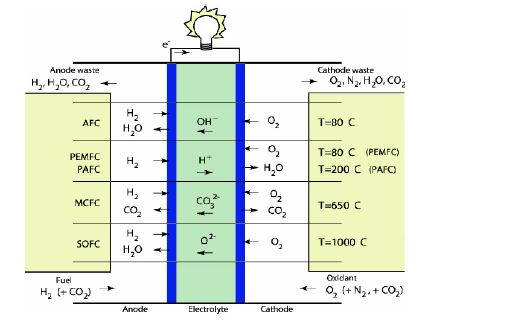
\includegraphics{Figures/Figure1}
\caption{fuel cell types and their respective operating temperatures
\cite{stefanopoulou_mechatronics_nodate}}
\end{figure}
\begin{figure}[!h]
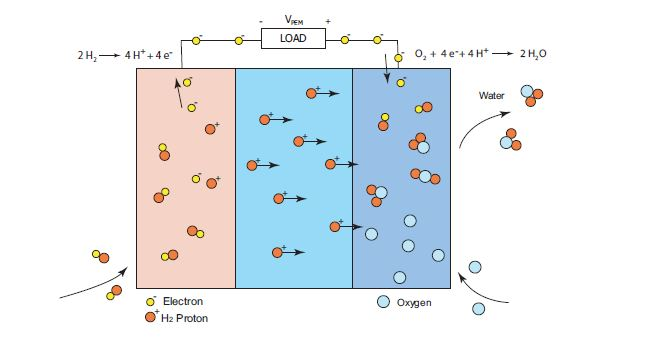
\includegraphics{Figures/Figure2}
\caption{Fuel Cell Reactions
\cite{pukrushpan_modeling_2003}}
\end{figure}
\paragraph{}Fuel cells convert chemical energy sources directly to electricity. A fuel cell consists of an electrolyte sandwiched between two electrodes. The electrolyte has a special property which allows protons to pass through while blocking electrons. Hydrogen gas passes over one electrode, i.e. an anode, and with the help of a catalyst, separates into electrons and hydrogen protons.
\begin{equation}
$$2H_{2}\rightarrow 4H^{+} + 4e^{-}$$
\end{equation}
\paragraph{}The protons flow to the other cathode through the electrolyte while the electrons flow through an external circuit, thus creating electricity. The hydrogen protons and electrons combine with oxygen flow through the cathode, and produce water.
\begin{equation}
$$O_{2}+ 4H_{2} + 4e^{-} \rightarrow 2H_{2}O $$
\end{equation}
\paragraph{}The overall reaction of the fuel cell is given by:
\begin{equation}
$$2H_{2}+ O_{2} \rightarrow 2H_{2}O $$
\end{equation}

\subsection{Problem statement}
\paragraph{}As a measure to curb pollution due to the industrialization and transportation sectors, world governments are turning to alternative sources of energy. These alternative sources of energy should drastically reduce the pollution rates by cutting down emissions. Fuel cell technology is one such example of alternative sources of energy. A fuel cell uses the chemical energy of hydrogen or other fuels to cleanly and efficiently produce electricity. Moreover, fuel cells can operate at higher efficiencies than combustion engines and can convert the chemical energy in the fuel directly to electrical energy with efficiencies capable of exceeding 60\%. Fuel cells have lower or zero emissions compared to combustion engines.
\paragraph{}The various departments of energy, however,  have to work closely with national laboratories, universities, and industry partners to overcome critical technical barriers to fuel cell development. These barriers are cost, performance, and durability which are still key challenges in the fuel cell industry. 
\paragraph{}This design proposal seeks to provide a solution to improving the fuel cell’s performance by improving the robustness and efficiency of the Fuel Cell stack system for real world conditions through precise control of reactant flow and pressure, stack temperature, and membrane humidity\cite{stefanopoulou_mechatronics_nodate}.
\subsection{Objectives}
\subsubsection{Main Objectives}
\begin{enumerate}
\item To develop a Hydrogen Fuel cell control system.
\end{enumerate}
\subsubsection{Specific Objectives}
\begin{enumerate}
\item To design and additively manufacture a PEMFC prototype which can be adapted for domestic use and scaled for industrial applications.
\item To design and fabricate supporting control electronics for the Hydrogen Fuel Cell.
\item To achieve precise control of reactant flow and pressure, stack temperature, and membrane humidity.
\item To simulate and test alternative control strategies for the Hydrogen fuel cell. 
\end{enumerate}
\subsection{Justification of the study}
\paragraph{}Additive manufacturing offers the ability to produce intricate products and parts with lower development costs, shorter lead times, less energy consumed during manufacturing as well as less material waste. This method can be used to manufacture delicate components such as the bipolar plates with elimination of the risks involved such as breakage of brittle graphene material during production.     
\paragraph{}Precise control of reactant flow and pressure, stack temperature, and membrane humidity will increase the fuel cell’s robustness as well as efficiency \cite{stefanopoulou_mechatronics_nodate}\cite{gonzatti_proposal_2017}\cite{thanapalan_model_nodate}.
\paragraph{}The goal of this research is to develop physic-based dynamic models of fuel cell systems and fuel processor systems and then apply multivariable control techniques to study their behavior. The analysis will give insight into the control design limitations and provide guidelines for the necessary controller structure and system re-design.